\documentclass[11pt,a4paper]{article}
\usepackage[T1]{fontenc}
\usepackage[utf8]{inputenc}
\usepackage{lmodern}
\usepackage[margin=2.3cm]{geometry}
\usepackage{amsmath,amssymb,booktabs,graphicx,longtable,float}
\usepackage{microtype,xcolor,caption}
\usepackage[hidelinks]{hyperref}
\usepackage{enumitem}
\usepackage[section]{placeins}
\setlength{\parskip}{0.4em}
\setlength{\parindent}{0pt}
\setlist{nosep,leftmargin=*}
\captionsetup{font=small,labelfont=bf}
\definecolor{navy}{HTML}{172C49}
\graphicspath{{figures/}}
\newcommand{\EEG}{\textsc{eeg}}
\newcommand{\R}{\mathbb{R}}
\newcommand{\ind}{\mathbf{1}}

\begin{document}
\hypersetup{pageanchor=false}
\begin{titlepage}
\centering
\vspace*{1.6cm}
{\Large SF2956 Topological Data Analysis\par}
\vspace{2.3cm}
{\Huge\bfseries\color{navy} Topological Analysis of\\[0.35cm]Motor Imagery EEG Data\par}
\vspace{1cm}
{\Large Frequency-specific dependence networks\\from nine participants\par}
\vspace{2cm}
{\large Galya Gadzhalova\par}
% Add any additional group authors here before submission.
\vfill
{\large Project report\\6 November 2026\par}
\vspace{1cm}
{\small BCI Competition IV, data set 2a / BNCI 001-2014\par}
\end{titlepage}
\pagenumbering{roman}
\hypersetup{pageanchor=true}
\tableofcontents
\clearpage
\pagenumbering{arabic}

\begin{abstract}
We examined whether imagined left-hand, right-hand, feet and tongue movements have different topological signatures in EEG sensor-dependence networks. Training recordings from all nine participants in BCI Competition IV data set 2a were analysed. After original artifact exclusions, 2,328 of 2,592 trials remained; balancing the four conditions within each participant selected 2,224 trials. Trial-pooled Welch coherence in mu (8--12 Hz bins) and beta (13--30 Hz bins) bands was transformed to channel dissimilarity, followed by weighted flag filtrations, $H_0$/$H_1$ persistence and standard stable ranks. Individual movement differences were visible, particularly in A01, but their ordering and size varied across people. Exploratory permutation-calibrated Friedman tests of finite total persistence did not detect a group-level movement effect after Holm correction (adjusted $p\geq0.9816$). A common sample size of 49 trials per condition gave the same inferential conclusion. The findings demonstrate a reproducible approach to frequency-specific EEG topology, while providing insufficient evidence for a consistent movement effect in the tested scalar summaries. They do not establish equality of the full networks or barcodes.
\end{abstract}


\section{Objective and research question}
This project asks: \emph{Do different imagined movements produce different topological signatures in frequency-specific EEG dependence networks, and are those patterns consistent across participants?} The four conditions are imagined left-hand, right-hand, feet and tongue movements. The analysis first compares conditions within each participant, then examines consistency across nine participants.

The object being analysed is a network of EEG sensors. Each vertex represents a channel; edge weights describe spectral dependence between two channels during one movement condition. Persistent homology follows the network over a range of thresholds, and stable ranks summarize the resulting barcodes. The purpose is to describe and compare dependence structure. No movement classifier, prediction accuracy, anatomical source localization or causal communication model is fitted.

El Yaagoubi Bourakna, Chung and Ombao motivate the use of coherence-derived dissimilarities for multivariate time-series topology \cite{bourakna2022}. This project adapts that approach to trial-pooled Welch spectra and the course's barcode/stable-rank framework. It is not an exact reproduction of the paper's kernel-smoothed periodogram or its application. The supplied lecture handouts connect single-linkage components, barcodes, simplicial complexes and homology \cite{lectures}; the standard-contour convention used here is also specified by Chach\'olski and Riihim\"aki \cite{chacholski2020}.

\section{Data and observation units}
\subsection{Dataset}
The data are the nine training-session MATLAB files \texttt{A01T.mat}--\texttt{A09T.mat} from BNCI 001-2014, originally released as BCI Competition IV data set 2a \cite{bnci,brunner2008}. Each participant has four movement-imagery classes, six task runs and 48 trials per run, giving 288 original trials per training session. The available evaluation sessions are not used here. There are 22 EEG and three electrooculography (EOG) channels, sampled at 250 Hz. The original acquisition used a left-mastoid reference, a 0.5--100 Hz bandpass and a 50 Hz notch \cite{brunner2008}.

The cue starts two seconds after the trial marker and imagery continues until six seconds. Thus the analysed interval is $[2,6)$ seconds relative to the trial marker, or $[0,4)$ seconds after the cue. Calibration blocks have no task trials and are skipped. A04 has a different calibration-block structure, so blocks are selected by their trial markers rather than their positions \cite{brunner2008}.

\begin{table}[htbp]
\centering
\caption{Variables used from each MATLAB recording block.}
\begin{tabular}{ll}
\toprule Variable & Meaning in this analysis \\
\midrule
\texttt{X} & Samples $\times$ 25 signal channels \\
\texttt{trial} & Trial-start sample markers, originally one-based \\
\texttt{y} & Movement labels: 1 left, 2 right, 3 feet, 4 tongue \\
\texttt{artifacts} & Original trial-level artifact indicators \\
\texttt{fs} & Sampling frequency in Hz \\
\texttt{classes} & Class names used to verify the label order \\
\bottomrule
\end{tabular}
\end{table}

\subsection{Blocks, channels and trials}
A \emph{block} is a continuous recording run. A \emph{channel} is one sensor's time series. A \emph{trial epoch} is the four-second window extracted for one imagery instruction. Each retained trial therefore has shape $1000\times22$: 1,000 time samples and 22 EEG channels. These samples, channels and repeated trials are nested within participants. The independent units for the group comparison are the nine participants, not the individual time points or channels.

\section{Data preparation}
\subsection{Extraction and exclusions}
For every task block, MATLAB sample indices are converted to zero-based Python indices. An epoch starts 500 samples after its trial marker and contains 1,000 samples. Only EEG columns 1--22 enter the network analysis. EOG channels are retained for visual inspection. Original block and trial identifiers are kept throughout so every selected or excluded trial can be traced.

Trials with a nonzero dataset artifact flag or a nonfinite EEG value are excluded. The code stops if a retained channel is flat or an epoch is incomplete, rather than assigning an arbitrary coherence value. All nine files passed these additional checks; the observed exclusions came from the dataset artifact flags. No additional time-domain filtering, ICA, re-referencing or baseline subtraction is applied. Mean removal occurs inside each Welch window, as described below. This is a consistent baseline preparation protocol, not a claim that every retained trial is artifact-free.

\subsection{Amplitude review}
For trial $r$, define its largest channel peak-to-peak amplitude as
\begin{equation}
 A_r=\max_{i=1,\ldots,22}\{\max_t X_{ri}(t)-\min_t X_{ri}(t)\}.
\end{equation}
Within each participant, flag $A_r>\operatorname{median}(A)+6\times1.4826\times\operatorname{MAD}(A)$, where MAD is the median absolute deviation from the median. These are \emph{review candidates}; they remain in the primary analysis. EEG and EOG plots are saved for each flagged trial. A sensitivity scenario temporarily removes all candidates and recalculates the all-retained coherence matrices. The mean absolute matrix change is calculated over the $\binom{22}{2}=231$ unique off-diagonal EEG pairs; the maximum reports the most changed pair. These changes are neither $p$-values nor tests of neural origin.

\subsection{Balancing and scale}
For participant $s$, let $n_s$ be the smallest retained trial count among the four movements. Randomly select $n_s$ trials without replacement from each class using seed 42. This matches the original A01 notebook and prevents movement comparisons from using different numbers of spectral realizations within a participant. A secondary analysis uses 49 trials per movement for every participant, the smallest available count in the entire dataset. This checks sensitivity to different sample sizes across people; it is one seeded selection.

EEG is not z-scored across people. Coherence is dimensionless, and a fixed nonzero scale multiplier applied to a channel across its trials cancels between its numerator and denominator. This property does not remove differences in reference, noise, trial amplitudes, anatomy or signal mixing. Participants' raw recordings are never concatenated or averaged together.

\section{Analysis methods}
\subsection{From EEG traces to channel dissimilarities}
Each trial is analysed separately using Welch estimation with 250-sample periodic Hann windows, 125-sample overlap, a 250-point Fourier transform and constant detrending. A four-second epoch yields seven overlapping windows and 1-Hz frequency spacing. These overlapping windows are not seven independent observations. Spectra are averaged over windows, then pooled over selected trials within one participant and movement. The implementation uses SciPy's Welch and cross-spectral-density functions \cite{scipycsd}.

Let $\widehat S^{(r)}_{ij}(f)$ denote the complex cross-spectrum for channels $i,j$ in trial $r$. For movement $m$ with $n_{sm}$ selected trials,
\begin{align}
 \overline S_{ij,sm}(f)&=\frac{1}{n_{sm}}\sum_{r\in\mathcal I_{sm}}\widehat S^{(r)}_{ij}(f),\\
 \widehat C_{ij,sm}(f)&=\frac{|\overline S_{ij,sm}(f)|^2}
 {\overline S_{ii,sm}(f)\overline S_{jj,sm}(f)}.
\end{align}
The complex spectra are averaged \emph{before} taking the squared magnitude. Averaging raw EEG traces or averaging trial-specific coherence values would produce a different estimator.

Use frequency bins $F_\mu=\{8,9,10,11,12\}$ Hz and $F_\beta=\{13,14,\ldots,30\}$ Hz. The band-specific dissimilarity is
\begin{equation}
 D^{(B)}_{ij,sm}=1-\frac{1}{|F_B|}\sum_{f\in F_B}\widehat C_{ij,sm}(f),
 \qquad D^{(B)}_{ii,sm}=0.
\end{equation}
A small value indicates stronger estimated dependence in that band. Each matrix is symmetric, finite and bounded by zero and one. It compares channels, not trials or people. The primary analysis produces $9\times4\times2=72$ matrices of size $22\times22$.

\subsection{Filtration and persistent homology}
For each matrix, form the weighted flag complex
\begin{equation}
 K_\epsilon=\{\sigma\subseteq\{1,\ldots,22\}:\sigma\ne\varnothing,
 D_{ij}\leq\epsilon\text{ for all }i,j\in\sigma\}.
\end{equation}
All vertices exist at zero. Edges enter as their dissimilarities are reached; whenever all edges of a triangle exist, its interior is included. Larger cliques are treated similarly. As $\epsilon$ increases, complexes are nested. The transformation $1-C$ need not satisfy the triangle inequality, but this flag construction remains valid. Metric-space stability theorems should not automatically be applied to these matrices.

Ripser computes homology over $\mathbb F_2$ in dimensions 0 and 1, with maximum threshold 1 \cite{ripser}. $H_0$ tracks connected components merging; $H_1$ tracks loops before they become boundaries of filled simplices. A barcode interval $[b,d)$ records the birth and death thresholds of a feature. Thresholds and lifespans are dimensionless, not time in seconds. Since every edge has entered by 1, there is one essential (infinite) $H_0$ interval and no infinite $H_1$ intervals. The finite $H_0$ death thresholds are independently checked against minimum-spanning-tree edge weights.

\subsection{Stable ranks and two kinds of summary}
With the standard contour $C(b,t)=b+t$, the stable rank is
\begin{equation}
 R_q(t)=\sum_{[b,d)\in\mathcal B_q}\ind\{d-b>t\},\qquad q\in\{0,1\}.
\end{equation}
It counts features whose lifespans strictly exceed the cutoff $t$ \cite{chacholski2020}. The infinite $H_0$ interval is retained, so $R_0$ eventually equals 1. $R_1$ eventually equals 0. For $H_0$, all births are zero, so the curve also describes the component count along the edge-threshold filtration. For $H_1$, a lifespan cutoff is distinct from a filtration threshold.

Two movement curves are compared within the same participant, band and homology by
\begin{equation}
 L_1(R_a,R_b)=\int_0^\infty |R_a(t)-R_b(t)|\,dt.
\end{equation}
The code integrates exactly over the union of barcode-lifespan breakpoints. Equal essential $H_0$ tails cancel. A larger value means more different lifespan distributions. The resulting $4\times4$ movement-comparison matrix differs from the $22\times22$ channel dissimilarity matrix. Stable ranks can lose information: different barcode birth positions can produce the same lifespan summary.

The scalar finite total persistence is $T_q=\sum_{d<\infty}(d-b)$. It equals $\int(R_0-1)$ for $H_0$ and $\int R_1$ for $H_1$. Larger $T_0$ means component mergers generally require larger dissimilarity thresholds. Larger $T_1$ can reflect more loops, longer loops or both; it does not directly imply greater activation or better brain function.

\subsection{Sensitivity and group analysis}
Repeat within-participant balancing 20 times using seeds 100--119. Re-estimate matrices and persistence for each selection. Plot pointwise medians and observed minimum--maximum ranges of stable ranks on a 0.0005-spaced display grid. Exact curve distances still use barcode breakpoints. Overlapping selections are dependent; their ranges are not confidence intervals. The smallest class is fully retained in every selection, which can make its curve identical across repetitions.

Across participants, summarize the six within-person movement-pair distances by their medians and show paired finite total persistence for each condition. An exploratory four-condition omnibus comparison uses the Friedman rank statistic for $T_q$ separately in the two bands and homology dimensions. Under the null of exchangeable movement labels within participants, randomly permute the four labels independently within each participant 99,999 times (seed 2026). Report
\begin{equation}
 p=\frac{1+\#\{Q_{\rm perm}\geq Q_{\rm observed}\}}{100000}.
\end{equation}
The statistic is tie-corrected and checked against SciPy; its asymptotic chi-squared $p$-value is not used because this is a small repeated-measures dataset \cite{friedman}. Holm adjustment is applied across the four primary tests. Kendall's $W=Q/(9\times3)$ describes consistency of condition ranks. The common-count sensitivity repeats the same test family separately. These are exploratory tests of one scalar summary, not comprehensive tests of barcode equality or of every visible curve separation. A descriptive feet/tongue-minus-hands contrast is motivated by the earlier A01 plot and is not treated as a pre-specified confirmatory hypothesis.

\section{Results}
\subsection{Retained trials and quality checks}

All 2,592 original trials were successfully segmented. The dataset artifact flags excluded 264 trials (10.2\%), leaving 2,328. No additional nonfinite, incomplete or flat-channel failures were observed. The balanced primary analysis used 49--67 trials per movement depending on participant (Table~\ref{tab:trials}); its total of 2,224 trials is smaller than the retained total because balancing discards surplus trials. A04 had seven recording blocks, including six task blocks, whereas the other files had nine blocks.

\begin{table}[htbp]\centering

\caption{Trial counts after the original artifact exclusions. LH/RH are left/right hand. Review candidates remain included in the main analysis.}\label{tab:trials}

\small\begin{tabular}{lrrrrrrrr}\toprule

Participant & Excluded & Retained & LH & RH & Feet & Tongue & Each$^*$ & Review\\\midrule

A01T & 15 & 273 & 69 & 69 & 68 & 67 & 67 & 1 \\

A02T & 18 & 270 & 67 & 69 & 66 & 68 & 66 & 2 \\

A03T & 18 & 270 & 69 & 68 & 66 & 67 & 66 & 0 \\

A04T & 26 & 262 & 62 & 67 & 67 & 66 & 62 & 0 \\

A05T & 26 & 262 & 63 & 66 & 66 & 67 & 63 & 0 \\

A06T & 69 & 219 & 56 & 57 & 49 & 57 & 49 & 0 \\

A07T & 17 & 271 & 67 & 66 & 67 & 71 & 66 & 6 \\

A08T & 24 & 264 & 66 & 66 & 64 & 68 & 64 & 0 \\

A09T & 51 & 237 & 53 & 63 & 61 & 60 & 53 & 0 \\

\bottomrule\end{tabular}

\par\smallskip\footnotesize $^*$Trials per movement in the balanced primary analysis (seed 42).

\end{table}

\subsection{A01: interpreting the original example}
The original A01 results were reproduced. All eight A01 networks had 22 $H_0$ intervals: 21 finite intervals and one infinite component. In the mu band, the numbers of $H_1$ intervals were 7, 8, 4 and 4 for left hand, right hand, feet and tongue, respectively. More intervals did not necessarily imply longer persistence: the longest mu $H_1$ lifespans were 0.0332, 0.0372, 0.0801 and 0.0829 in that order. Thus feet and tongue had fewer loops but some longer-lived ones (Figure~\ref{fig:a01}).

At a mu lifespan cutoff of 0.10, A01's $H_0$ stable ranks were 5, 5, 10 and 14. Because all $H_0$ births occur at zero, this also means that at edge threshold 0.10 the hand networks had fewer remaining components than the feet/tongue networks. This is a statement about how quickly these sensor networks connect as weaker dependencies are admitted; it does not show that one movement activates more brain regions.

\begin{figure}[htbp]
\centering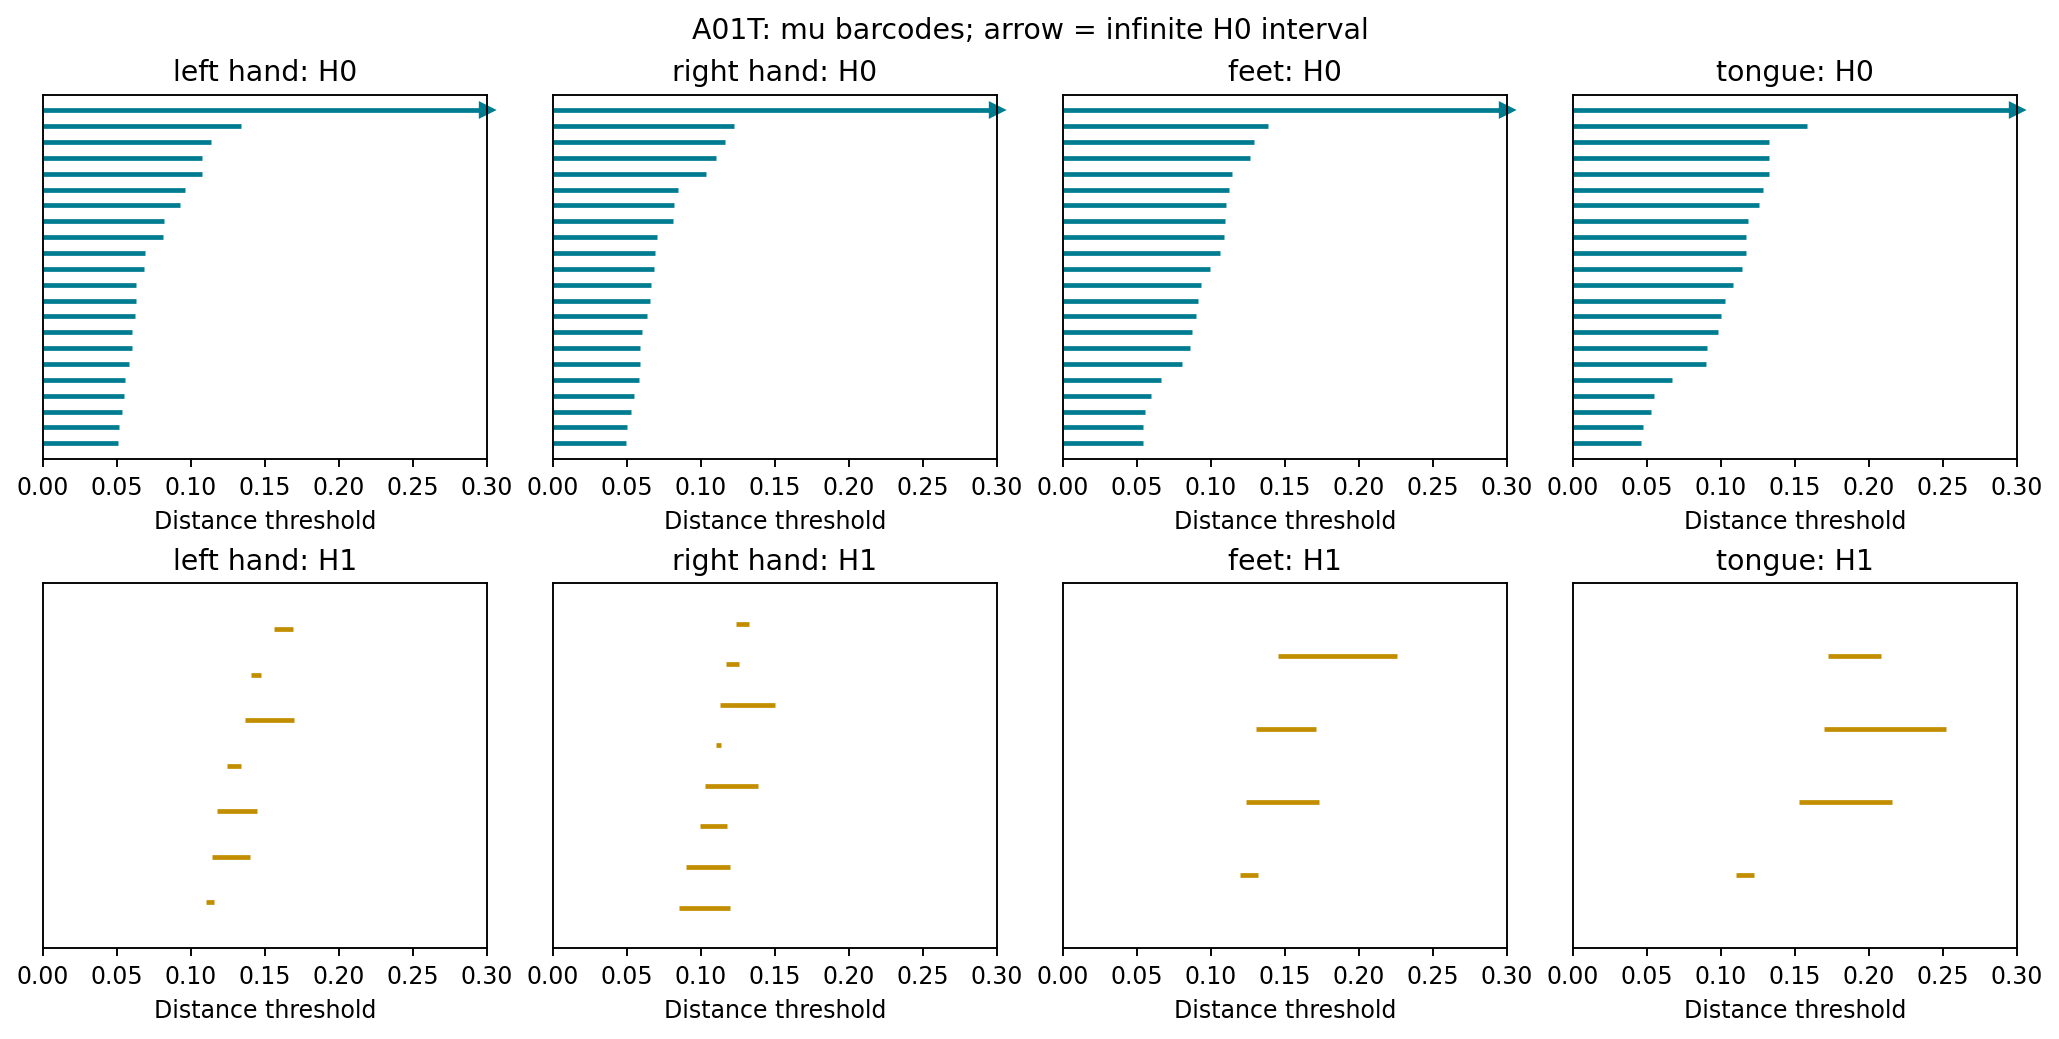
\includegraphics[width=\linewidth]{A01_barcodes_mu.png}
\caption{A01 mu-band barcodes for the seed-42 balanced selection (67 trials per movement). The arrow marks the essential $H_0$ interval. Blue/ochre lines encode threshold intervals, not EEG waveforms. The feet and tongue $H_1$ barcodes have fewer but longer-lived loops than the hand barcodes.}\label{fig:a01}
\end{figure}

\subsection{Differences across participants}
The A01 separation was not representative of every participant (Figure~\ref{fig:allnine}). For example, several participants' mu $H_0$ curves overlap closely, while A06 has generally larger merge thresholds and A02 smaller thresholds. These subject-level differences motivate paired, within-participant comparisons.

\begin{figure}[htbp]
\centering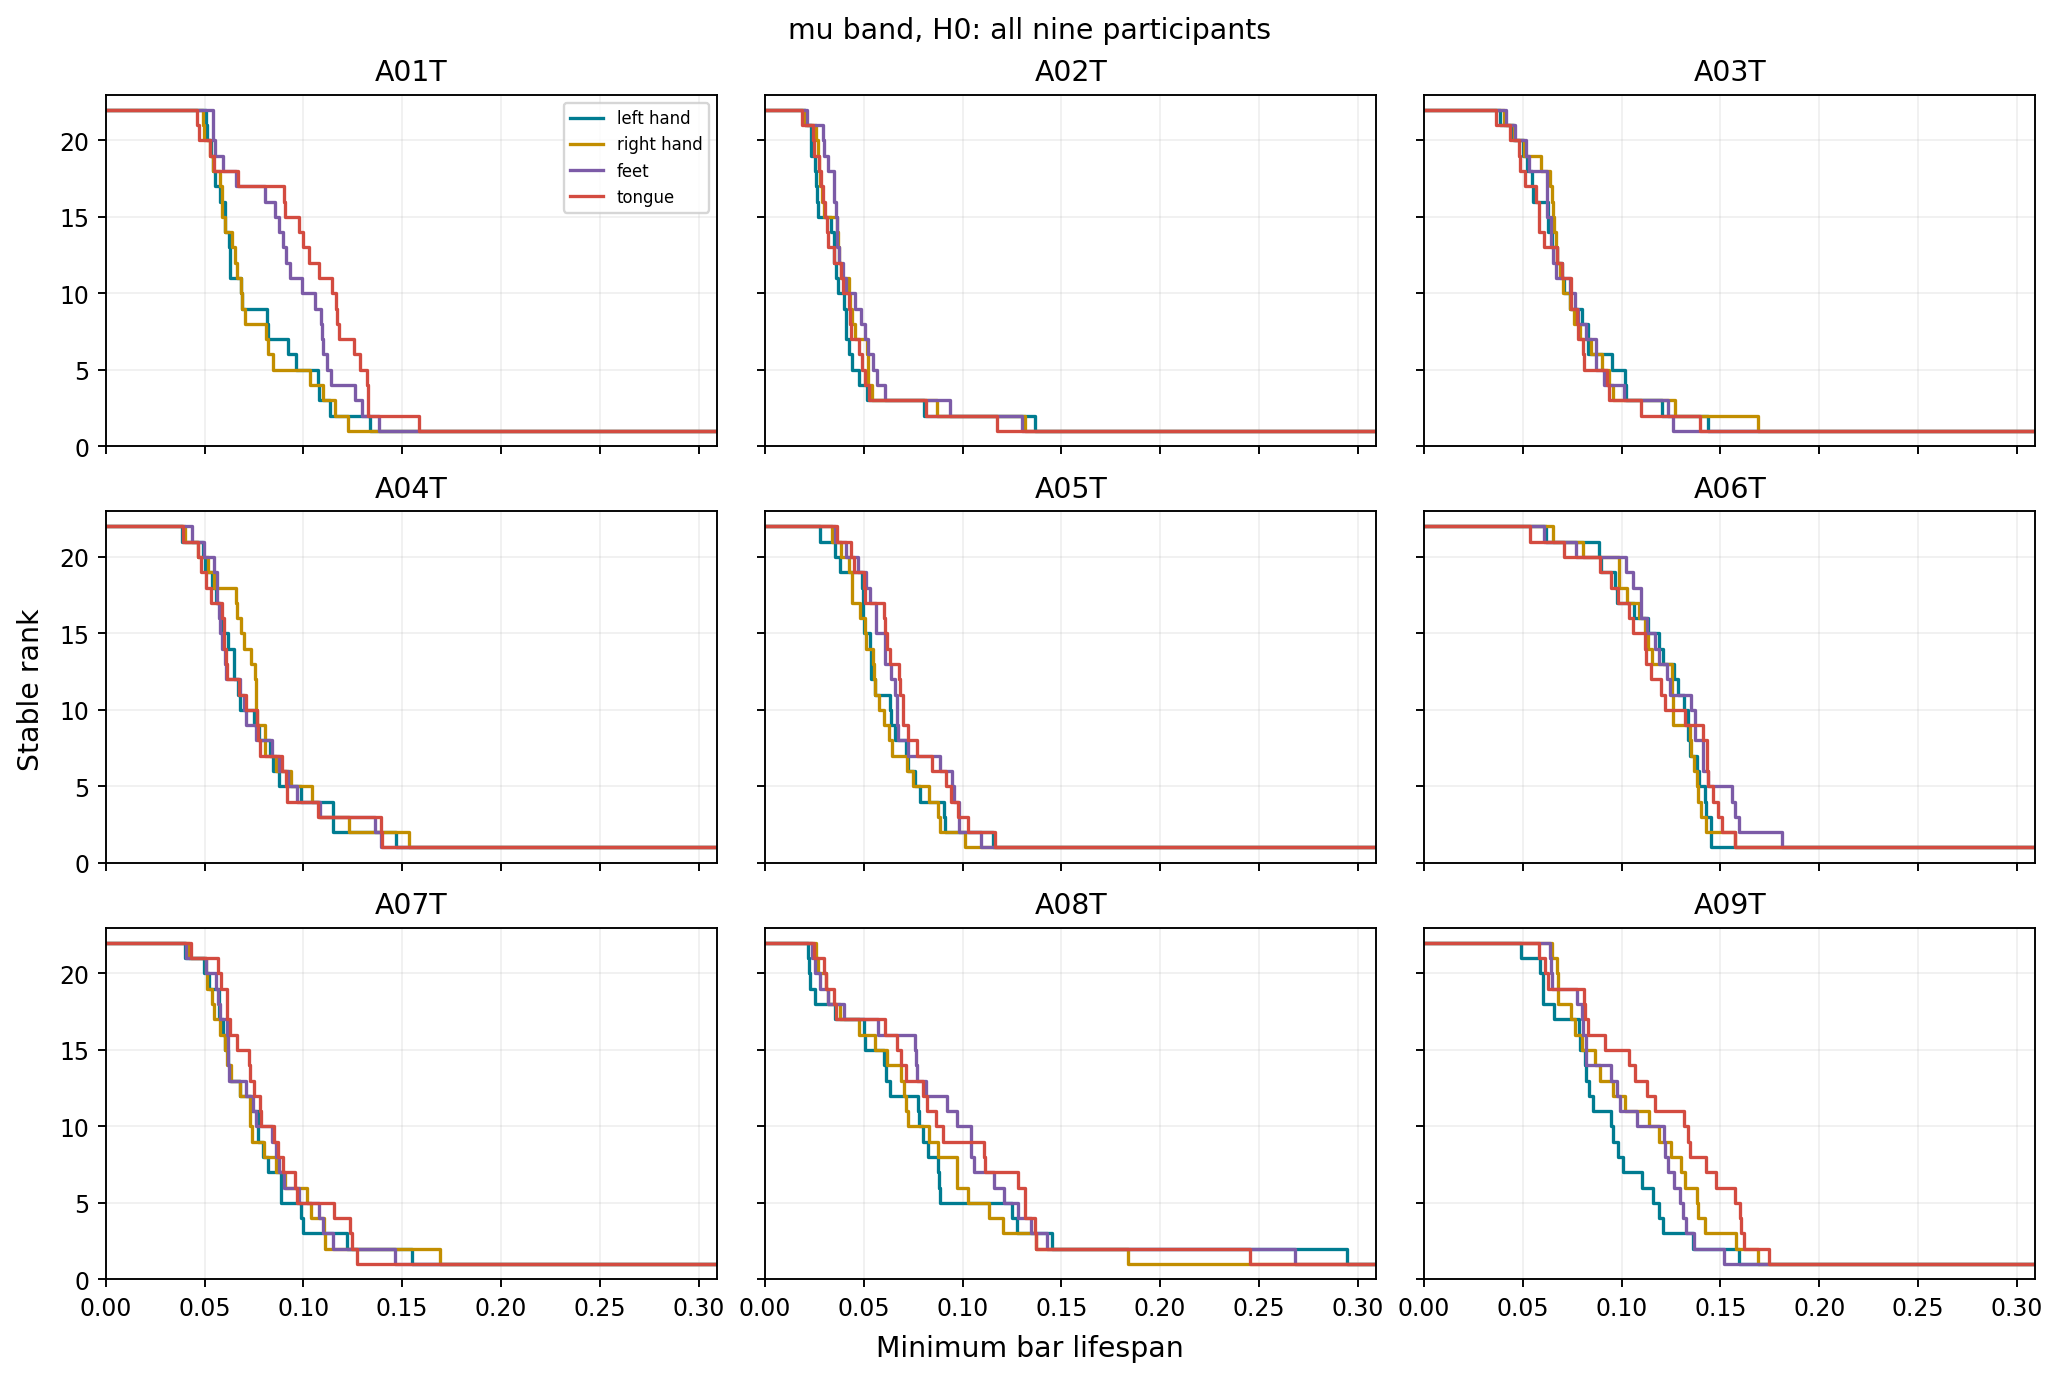
\includegraphics[width=\linewidth]{all_subjects_mu_H0.png}
\caption{Mu-band $H_0$ stable ranks for all nine participants on common axes. Colors have the same meaning in every panel. Movement differences and overall threshold scales vary between participants. The persistent level of one comes from the essential connected component.}\label{fig:allnine}
\end{figure}

Across participants, the median within-person mu $H_0$ L1 distance was 0.0822 for left versus right hand, compared with 0.1771 for left hand versus tongue and 0.1906 for right hand versus tongue (Figure~\ref{fig:l1}). These are descriptive separations of curves, not probabilities or test statistics. A larger distance does not indicate which movement has greater persistence.

The descriptive feet/tongue-minus-hands contrast in finite $H_0$ total persistence was positive in 7 of 9 participants in each band. Its median was 0.0713 in mu and 0.1008 in beta. For $H_1$, the direction was less consistent: positive in 5 of 9 participants in mu and 4 of 9 in beta. This contrast was motivated by A01 and is reported without a confirmatory significance claim.

\begin{figure}[htbp]
\centering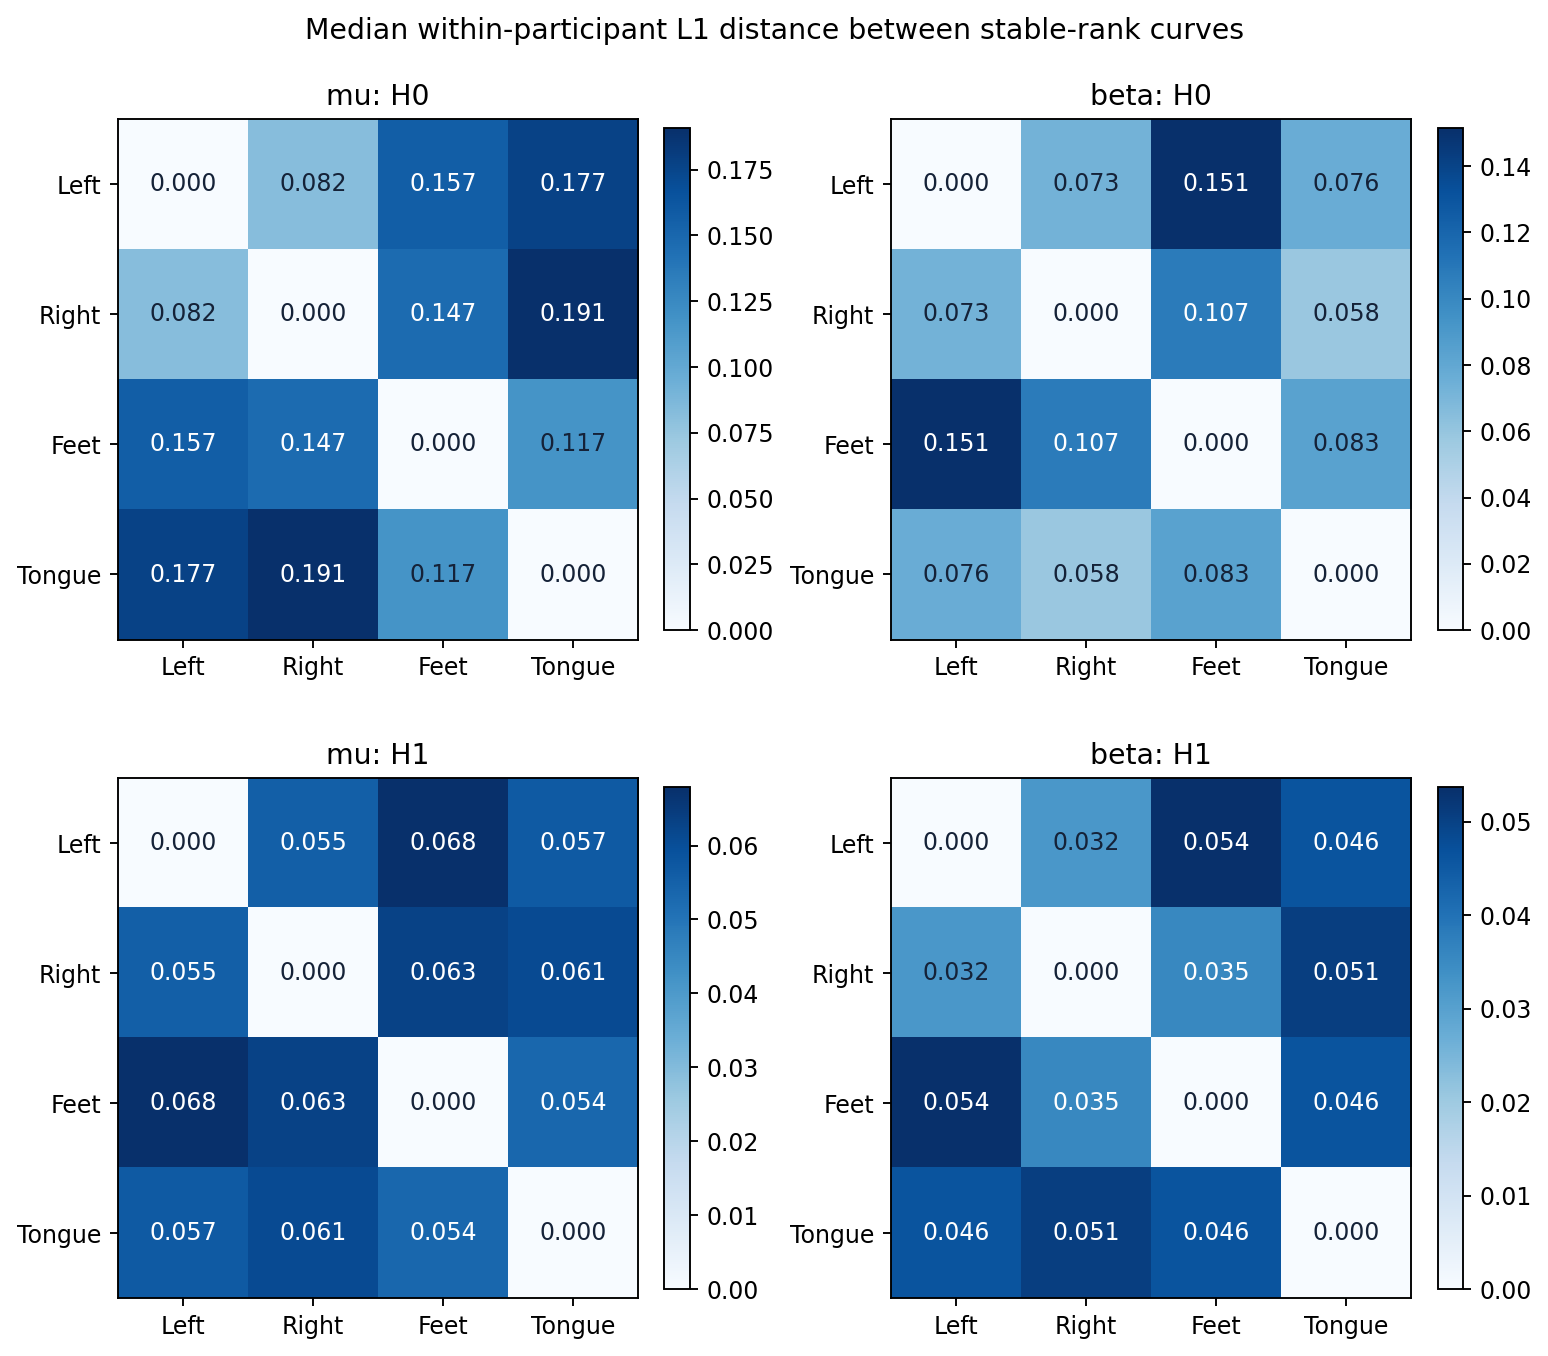
\includegraphics[width=0.83\linewidth]{group_pairwise_distances.png}
\caption{Across-participant medians of exact within-participant L1 distances between movement stable ranks. The four panels have separate color scales; comparisons must use the numbers. Zero diagonals compare each movement with itself. These are $4\times4$ movement comparisons, not channel matrices.}\label{fig:l1}
\end{figure}


\begin{table}[htbp]\centering

\caption{Median finite total persistence across nine participants; values are dimensionless. The infinite $H_0$ interval is excluded only from this scalar summary.}\label{tab:medians}

\begin{tabular}{llrrrr}\toprule

Band & Dimension & Left hand & Right hand & Feet & Tongue\\\midrule

Mu & $H_0$ & 1.5827 & 1.6236 & 1.6557 & 1.7327 \\

Mu & $H_1$ & 0.2489 & 0.2040 & 0.2166 & 0.2182 \\

Beta & $H_0$ & 2.2198 & 2.2375 & 2.2814 & 2.2935 \\

Beta & $H_1$ & 0.4086 & 0.3888 & 0.4016 & 0.3791 \\

\bottomrule\end{tabular}\end{table}

Table~\ref{tab:medians} and Figure~\ref{fig:paired} show that the central movement differences are modest relative to variation between participants. Medians of individual condition values need not equal medians of paired condition differences. Beta $H_0$ values are generally larger than mu $H_0$ values here, but no formal mu-versus-beta hypothesis test was specified; the bands use different frequency sets.

\begin{figure}[htbp]
\centering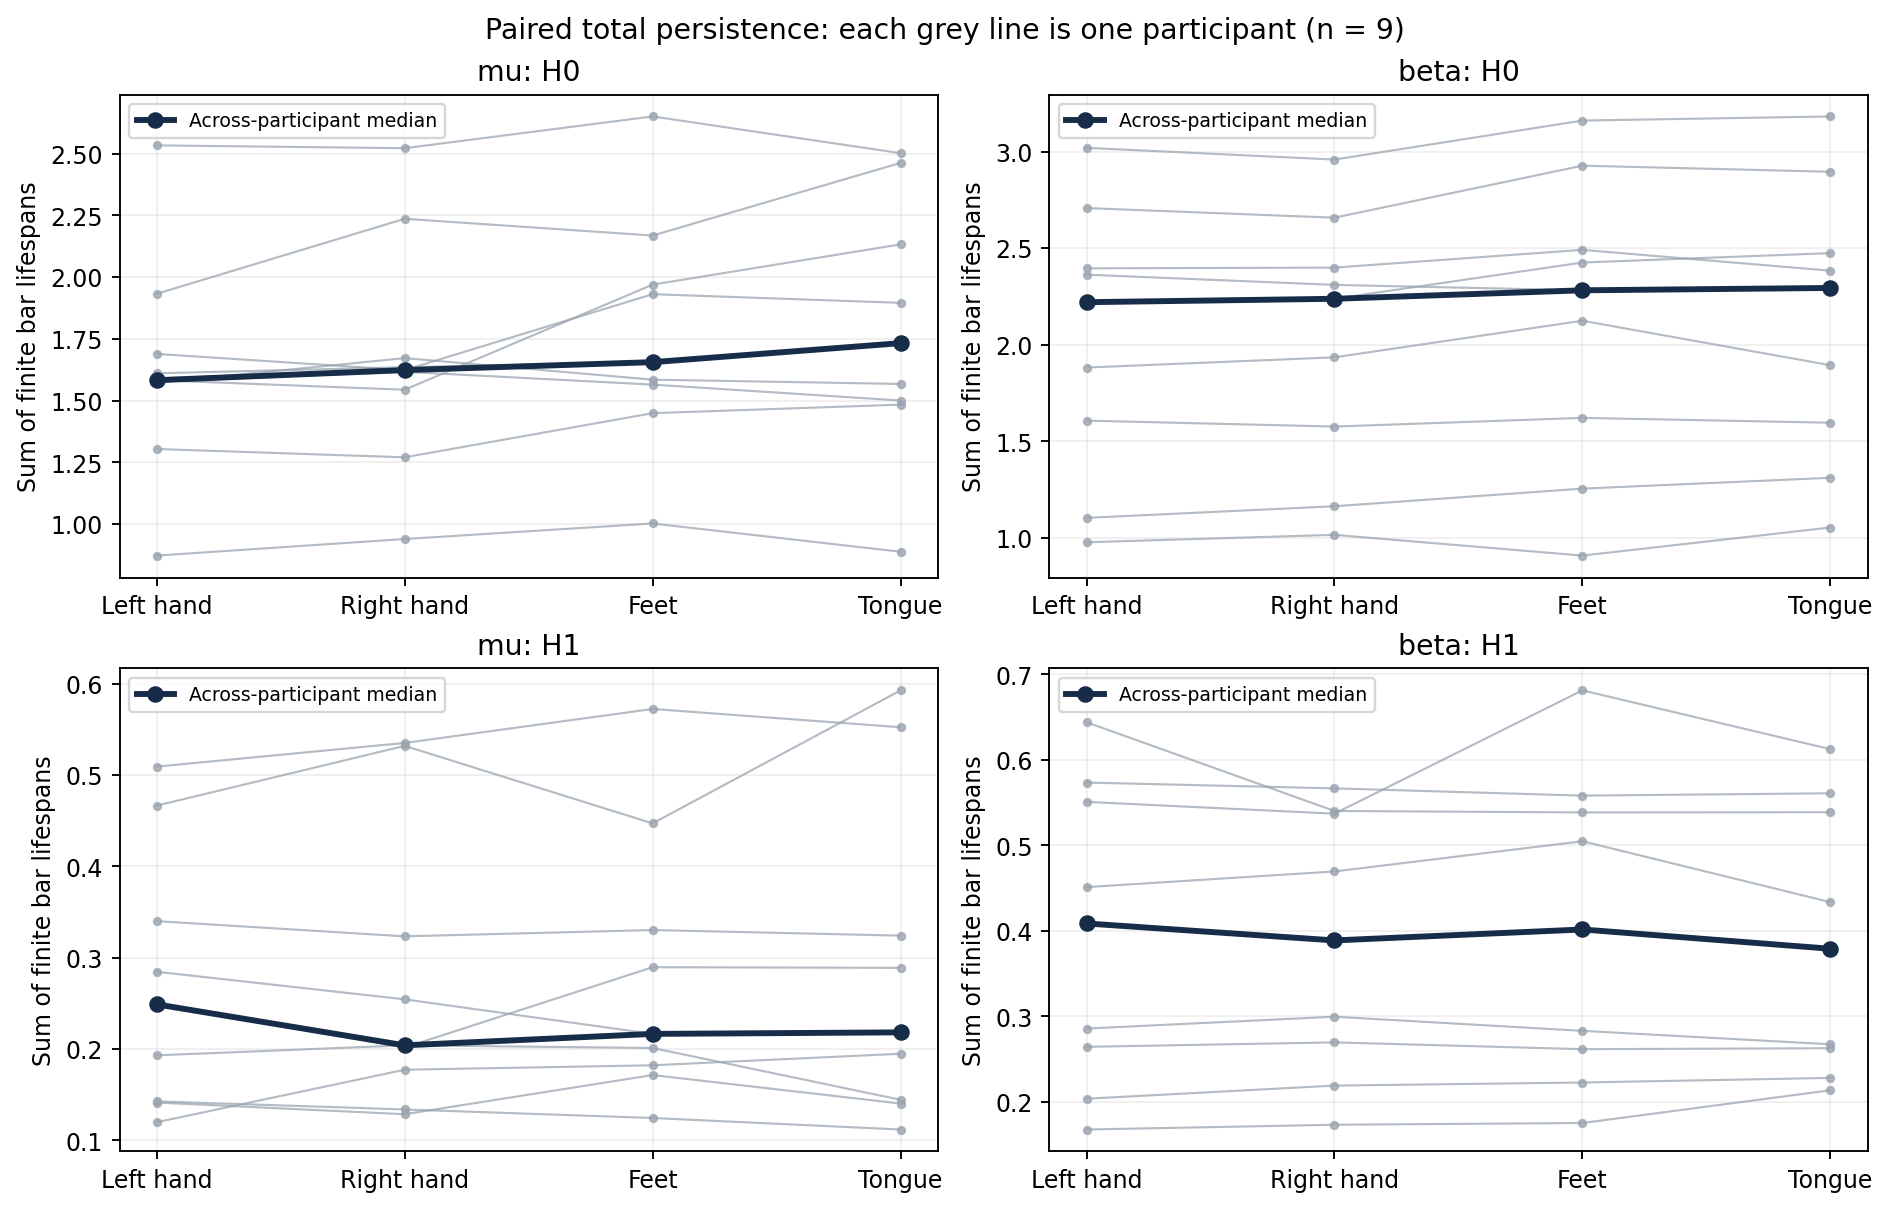
\includegraphics[width=\linewidth]{group_total_persistence.png}
\caption{Finite total persistence for the four movement conditions. Each grey line connects one participant's observations; the dark line is the pointwise median across participants. Curves that cross or change direction illustrate the inconsistent ordering of conditions.}\label{fig:paired}
\end{figure}

\subsection{Exploratory omnibus comparisons}
The four primary permutation tests did not detect a movement effect in finite total persistence after Holm adjustment (Table~\ref{tab:tests}). Rank agreement was low: Kendall's $W$ was about 0.160 for $H_0$ and 0.027--0.032 for $H_1$. This supports a cautious interpretation of the visual contrasts. A nonsignificant result does not prove that movements have identical networks or that the full stable-rank curves are equal: the tests use one finite-area summary and only nine participants.


\begin{table}[htbp]\centering

\caption{Exploratory primary tests of finite total persistence. Each test uses nine paired participants, four movement conditions and 99,999 within-participant label permutations.}\label{tab:tests}

\begin{tabular}{llrrrr}\toprule

Band & Dimension & Friedman $Q$ & Kendall $W$ & Permutation $p$ & Holm $p$\\\midrule

Mu & $H_0$ & 4.333 & 0.160 & 0.2455 & 0.9816 \\

Mu & $H_1$ & 0.867 & 0.032 & 0.8516 & 1.0000 \\

Beta & $H_0$ & 4.333 & 0.160 & 0.2454 & 0.9816 \\

Beta & $H_1$ & 0.733 & 0.027 & 0.8864 & 1.0000 \\

\bottomrule\end{tabular}\end{table}

Monte Carlo standard errors for the unadjusted primary $p$-values were approximately 0.0010--0.0014. This simulation uncertainty is small relative to their distance from 0.05. With 49 trials per movement for every participant (1,764 selected trials), the unadjusted $p$-values were 0.2901 (mu $H_0$), 0.7625 (mu $H_1$), 0.3053 (beta $H_0$) and 0.8184 (beta $H_1$); all four sensitivity-family Holm-adjusted values were 1.0000. Thus the absence of an omnibus signal in these summaries was unchanged by equalizing counts across participants.

\subsection{Sensitivity to trial selection and amplitude review}
All 180 repeated balanced selections completed. Table~\ref{tab:selection} summarizes exact L1 distances from the primary curve to each reselected curve, pooling the eight movement/band combinations and two homology dimensions within a participant. These pooled summaries are only a compact check; the separate curves and values are saved. A06 and A09 were more sensitive than the other participants. Their variation can be comparable with some movement-pair distances, so a small visual separation should not automatically be interpreted as a reliable movement signature.


\begin{table}[htbp]\centering

\caption{L1 change from the primary stable rank under 20 reselected balanced sets; each participant contributes 320 comparisons. These are sensitivity summaries, not confidence limits.}\label{tab:selection}

\begin{tabular}{lrr}\toprule Participant & Median change & Maximum change\\\midrule

A01T & 0.0053 & 0.0358 \\

A02T & 0.0043 & 0.0673 \\

A03T & 0.0043 & 0.0286 \\

A04T & 0.0096 & 0.0481 \\

A05T & 0.0068 & 0.0280 \\

A06T & 0.0237 & 0.1204 \\

A07T & 0.0063 & 0.0312 \\

A08T & 0.0054 & 0.0429 \\

A09T & 0.0210 & 0.1027 \\

\bottomrule\end{tabular}\end{table}

The amplitude rule identified nine review candidates: one in A01, two in A02 and six in A07. Removing these candidates temporarily changed only the conditions containing them. A01's tongue mu matrix changed by 0.001509 on average across unique channel pairs, with a maximum of 0.006213; its tongue beta changes were 0.000843 and 0.002298. The largest pairwise change anywhere in this check was 0.010402 (A02 tongue mu). The largest matrix mean change was 0.001740 (A02 tongue beta). Other participants had no additional amplitude-review exclusions in this scenario, giving zero changes by construction. These relatively small matrix changes do not establish artifact-free data or guarantee unchanged topological features; persistence was not recomputed for this amplitude-removal scenario.


\section{Discussion and limitations}
The analysis demonstrates that motor-imagery conditions can yield different dependence-network barcodes within a person. A01 is a clear example: feet and tongue have later component mergers and longer dominant mu loops than the hands. However, the ordering is not uniform across people. The group results therefore support an exploratory, participant-specific description rather than a general movement biomarker. Larger L1 distances for some movement pairs show differences in estimated curves but do not by themselves establish reproducibility or statistical significance.

Several limitations constrain interpretation:
\begin{enumerate}
\item \textbf{Small sample and limited scope.} Nine participants and one training session per participant provide limited power and no independent session-level replication. A01 was already explored when the project was developed; the subsequent summaries and tests are exploratory.
\item \textbf{Sensor mixing and residual artifacts.} Coherence can reflect common sources, volume conduction, reference effects and eye or muscle activity. Original artifact labels and amplitude review do not replace detailed artifact correction. The amplitude sensitivity check concerns matrices only. No causal or anatomical connections can be inferred from these sensor networks.
\item \textbf{Selection and sample size.} Artifact rejection differs across people and conditions, and retained trials need not be a random sample of all trials. Balancing removes surplus data. Repeated selections overlap heavily, and the smallest class is fixed; narrow ranges therefore do not demonstrate strong external reproducibility. The 49-trial check is a single selection.
\item \textbf{Spectral assumptions.} Four-second trials may contain cue-related transients and changing rhythms. One-second Welch windows and band pooling give an average dependence estimate that suppresses temporal and frequency detail. Pooling complex cross spectra also depends on consistency of phase relationships across trials. No sensitivity analysis of window length, band boundaries or reference was performed.
\item \textbf{Topological information loss.} Standard stable ranks discard birth locations. Finite total persistence compresses a whole curve to one number. The nonsignificant omnibus tests do not exclude differences in curve shape, detailed barcodes or specific channel connections. Long-lived features are not automatically neural signal, and short-lived features are not automatically noise.
\item \textbf{Inference assumptions.} Permutation calibration assumes exchangeability of movement summaries within a participant under the null and independence between participants. Trial rejection and temporal/run structure may weaken a randomization interpretation. Holm adjustment covers the four specified primary scalar tests, not every descriptive plot or post hoc interpretation. No held-out classification experiment was conducted.
\end{enumerate}

Useful next steps are replication in the evaluation sessions, more participants, documented artifact correction and sensitivity to spectral settings. A planned full-curve or barcode comparison could complement finite total persistence. If classification is later attempted, training/test separation must be defined at the participant or session level appropriate to the prediction question; overlapping trial selections must not be treated as independent train/test examples.


\section{Conclusion}
A complete, reproducible analysis was performed for all nine participants, from raw recording blocks through quality screening, balanced trial-pooled coherence, channel dissimilarities, persistent homology, stable ranks and group comparisons. The original A01 findings were reproduced and placed in the context of substantial between-participant variation. The four exploratory tests found no evidence of a consistent movement effect in finite total persistence after multiplicity correction; equalizing trial counts across participants did not change this conclusion. The project therefore establishes a practical way to describe EEG dependence-network topology, while the present data and summaries are insufficient to establish a generalizable movement-specific topological signature.


\section*{Reproducibility}
\addcontentsline{toc}{section}{Reproducibility}
The completed notebook contains the preparation, estimation, topology, repeated-selection and group-analysis code with executed outputs. Each participant's folder stores a trial audit, settings and source-file SHA-256, selected trial IDs, coherence/dissimilarity matrices, barcodes, stable-rank arrays, exact movement distances and figures. The group CSV files contain the values used in this report. Cached per-trial spectral matrices reproduce the original A01 implementation to a maximum absolute matrix difference of $4.44\times10^{-16}$; the A01 barcode counts and distance results also reproduce. The source files can be downloaded from the official links in the notebook. Raw data are not bundled in the project archive.

The executed software versions were numpy 2.3.5, scipy 1.17.0, ripser 0.6.15, matplotlib 3.10.8, pandas 2.2.3. Random seeds, source hashes and every subject-specific setting are stored in the accompanying results.


\begin{thebibliography}{9}
\bibitem{bnci} BNCI Horizon 2020. \emph{Four class motor imagery (001-2014)}. \url{https://bnci-horizon-2020.eu/database/data-sets}. Accessed 6 November 2026.
\bibitem{brunner2008} C. Brunner, R. Leeb, G. R. M\"uller-Putz, A. Schl\"ogl and G. Pfurtscheller. \emph{BCI Competition 2008 -- Graz data set A}. Dataset description. \url{https://lampx.tugraz.at/~bci/database/001-2014/description.pdf}.
\bibitem{bourakna2022} A. El Yaagoubi Bourakna, M. K. Chung and H. Ombao. \emph{Topological Data Analysis for Multivariate Time Series Data}. arXiv:2204.13799, 28 April 2022. \url{https://arxiv.org/abs/2204.13799}. Subsequently published in \emph{Entropy} 25(11), 1509 (2023).
\bibitem{chacholski2020} W. Chach\'olski and H. Riihim\"aki. \emph{Metrics and stabilization in one parameter persistence}. arXiv:1904.02905v2, 2020; \emph{SIAM Journal on Applied Algebra and Geometry} 4(1). Sections 5.3 and 8. \url{https://arxiv.org/abs/1904.02905}.
\bibitem{lectures} SF2956 Topological Data Analysis. Supplied lecture handouts 9--12: barcodes and stable ranks; simplicial complexes; Vietoris--Rips constructions; homology. Course materials.
\bibitem{scipycsd} SciPy developers. \emph{scipy.signal.csd and Welch spectral estimation}. \url{https://docs.scipy.org/doc/scipy/reference/generated/scipy.signal.csd.html}.
\bibitem{ripser} Ripser.py developers. \emph{ripser.ripser reference documentation}. \url{https://ripser.scikit-tda.org/en/latest/reference/stubs/ripser.ripser.html}.
\bibitem{friedman} SciPy developers. \emph{scipy.stats.friedmanchisquare reference documentation}. \url{https://docs.scipy.org/doc/scipy/reference/generated/scipy.stats.friedmanchisquare.html}.
\end{thebibliography}
\end{document}
